\section{Tutorial}

The aim of the tutorial mode is to show the user the variety of PIPS
abilities. At the begining, the chosen example is loaded, as is shown
in Figure~\ref{fig:tutorial_screen} (example ``Acca-2011'').

\begin{figure}[h!]
  \centering
  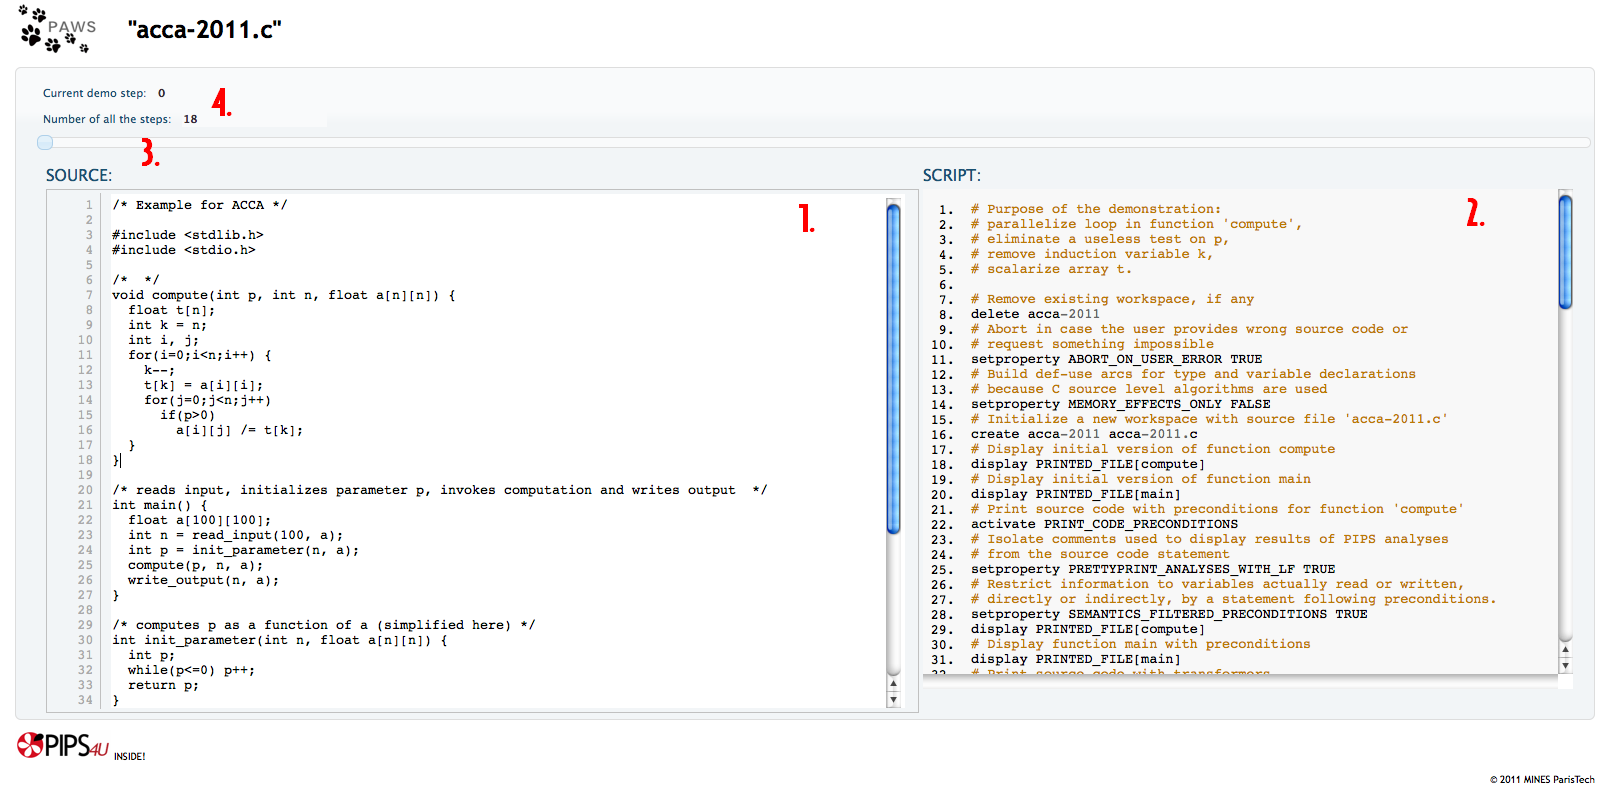
\includegraphics[width=0.8\textwidth]{reportCh4/tutorial_screen}
  \caption{``Acca-2011'' tutorial screen.}
  \label{fig:tutorial_screen}
\end{figure}

This mode does not require a significant interaction with the user -
the source code ({\bf 1.}) and the script with operations and comments
({\bf 2.}) are provided. The user only needs to change the current
step using the slider ({\bf 3.}). It is very flexible and stepping
does not have to be sequential: the user can go back or skip some
steps. The current step and the numbers of all steps are displayed
over the slider ({\bf 4.}).
